\documentclass[11pt,a4paper]{article}
\usepackage{graphicx}
\usepackage{isabelle,isabellesym}
\usepackage{amssymb}
\usepackage[utf8]{inputenc}
\usepackage{url}

% this should be the last package used
\usepackage{pdfsetup}


\urlstyle{rm}
\isabellestyle{it}
\pagestyle{myheadings}

\begin{document}

\title{Local Lexing}
\author{Steven Obua}
\maketitle

\begin{abstract}
This formalisation accompanies the paper Local Lexing\footnote{\url{https://arxiv.org/abs/1702.03277}}, which introduces a novel parsing concept of the same name. The paper also gives a high-level algorithm for local lexing as an extension of Earley's algorithm. This formalisation proves the algorithm to be correct with respect to its local lexing semantics. As a special case, this formalisation thus also contains a proof of the correctness of Earley's algorithm. The paper contains a short outline of how this formalisation is organised.
\end{abstract}

\tableofcontents

\begin{center}
  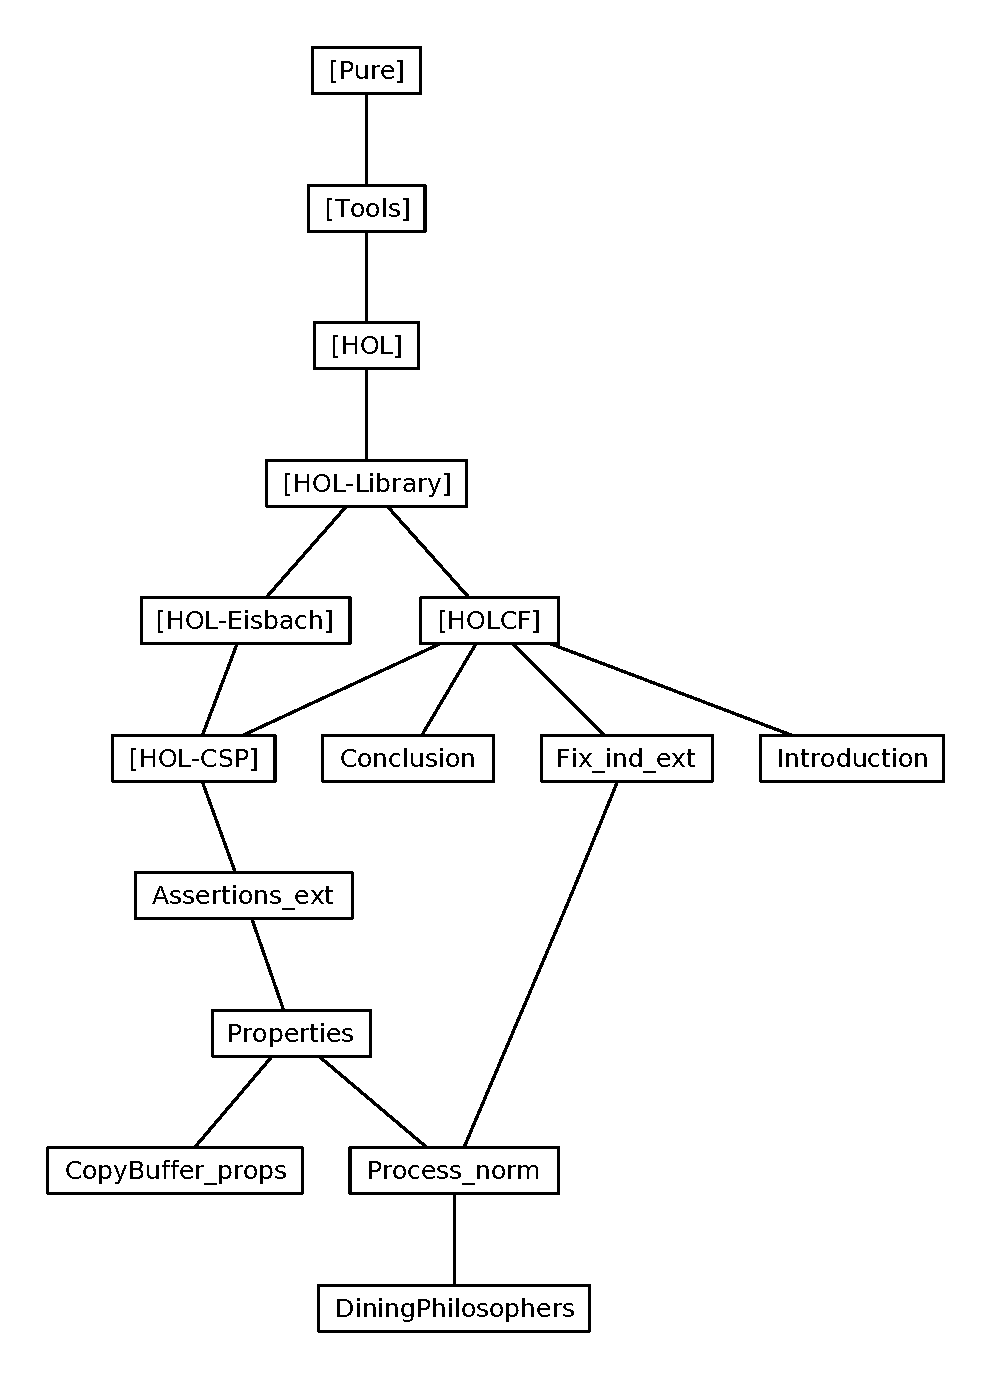
\includegraphics[scale=0.5]{session_graph}
\end{center}

\clearpage

\parindent 0pt\parskip 0.5ex
\input{session}

\end{document}
